% The next command tells RStudio to do "Compile PDF" on HSB.Rnw,
% instead of this file, thereby eliminating the need to switch back to HSB.Rnw 
% before building the paper.
%!TEX root = ../HSB.Rnw

\renewcommand{\arraystretch}{0.6}

\begin{landscape}
\begin{table}
\begin{center}
\caption{Previous rebound analysis frameworks. **** This table is not correct. We need to decide which
           frameworks to include and their characteristics. ---MKH ****}
\begin{tabular}{r c c}
  \toprule
                                             & \rot{\citet{Thomas:2013aa}} 
                                             & \rot{\citet{Borenstein:2015aa}} \\
  \midrule
  \multicolumn{1}{l}{\emph{Integrated effects, locations, and scales}}  &    &     \\
  Direct emplacement effect                  & \rating{10}     & \rating{90}       \\
  Embodied energy effect                     & \rating{20}     & \rating{80}       \\
  Maintenance and disposal effect            & \rating{30}     & \rating{70}       \\
  \midrule
  Direct substitution effect                 & \rating{40}     & \rating{60}       \\
  Indirect substitution effect               & \rating{50}     & \rating{50}       \\
  \midrule
  Direct income effect                       & \rating{60}     & \rating{40}       \\
  Indirect income effect                     & \rating{70}     & \rating{30}       \\
  \midrule
  Macro effect                               & \rating{80}     & \rating{20}       \\
  \midrule
  \multicolumn{1}{l}{\emph{3 planes}}               &    &     \\
  Energy                                     & \rating{90}     & \rating{10}       \\
  Expenditure                                & \rating{100}    & \rating{0}        \\
  Consumption                                & \rating{90}     & \rating{10}       \\
  \midrule
  \multicolumn{1}{l}{Detailed model of consumer preferences}   & \rating{80}   &  \rating{20}  \\
  \midrule
  \multicolumn{1}{l}{Non-marginal energy service price changes}   & \rating{80}   &  \rating{20}  \\
  \midrule
  \multicolumn{1}{l}{Operationalizable}      & \rating{70}   &  \rating{30}  \\
  \bottomrule
\end{tabular}
\label{tab:previous_frameworks}
\end{center}
\end{table}
\end{landscape}

% \renewcommand{\arraystretch}{1}

% \begin{table} 
%   \caption{Previous rebound analysis frameworks. **** This table is not correct. We need to decide which 
%            frameworks to include and their characteristics. ---MKH ****}
%   \centering
%   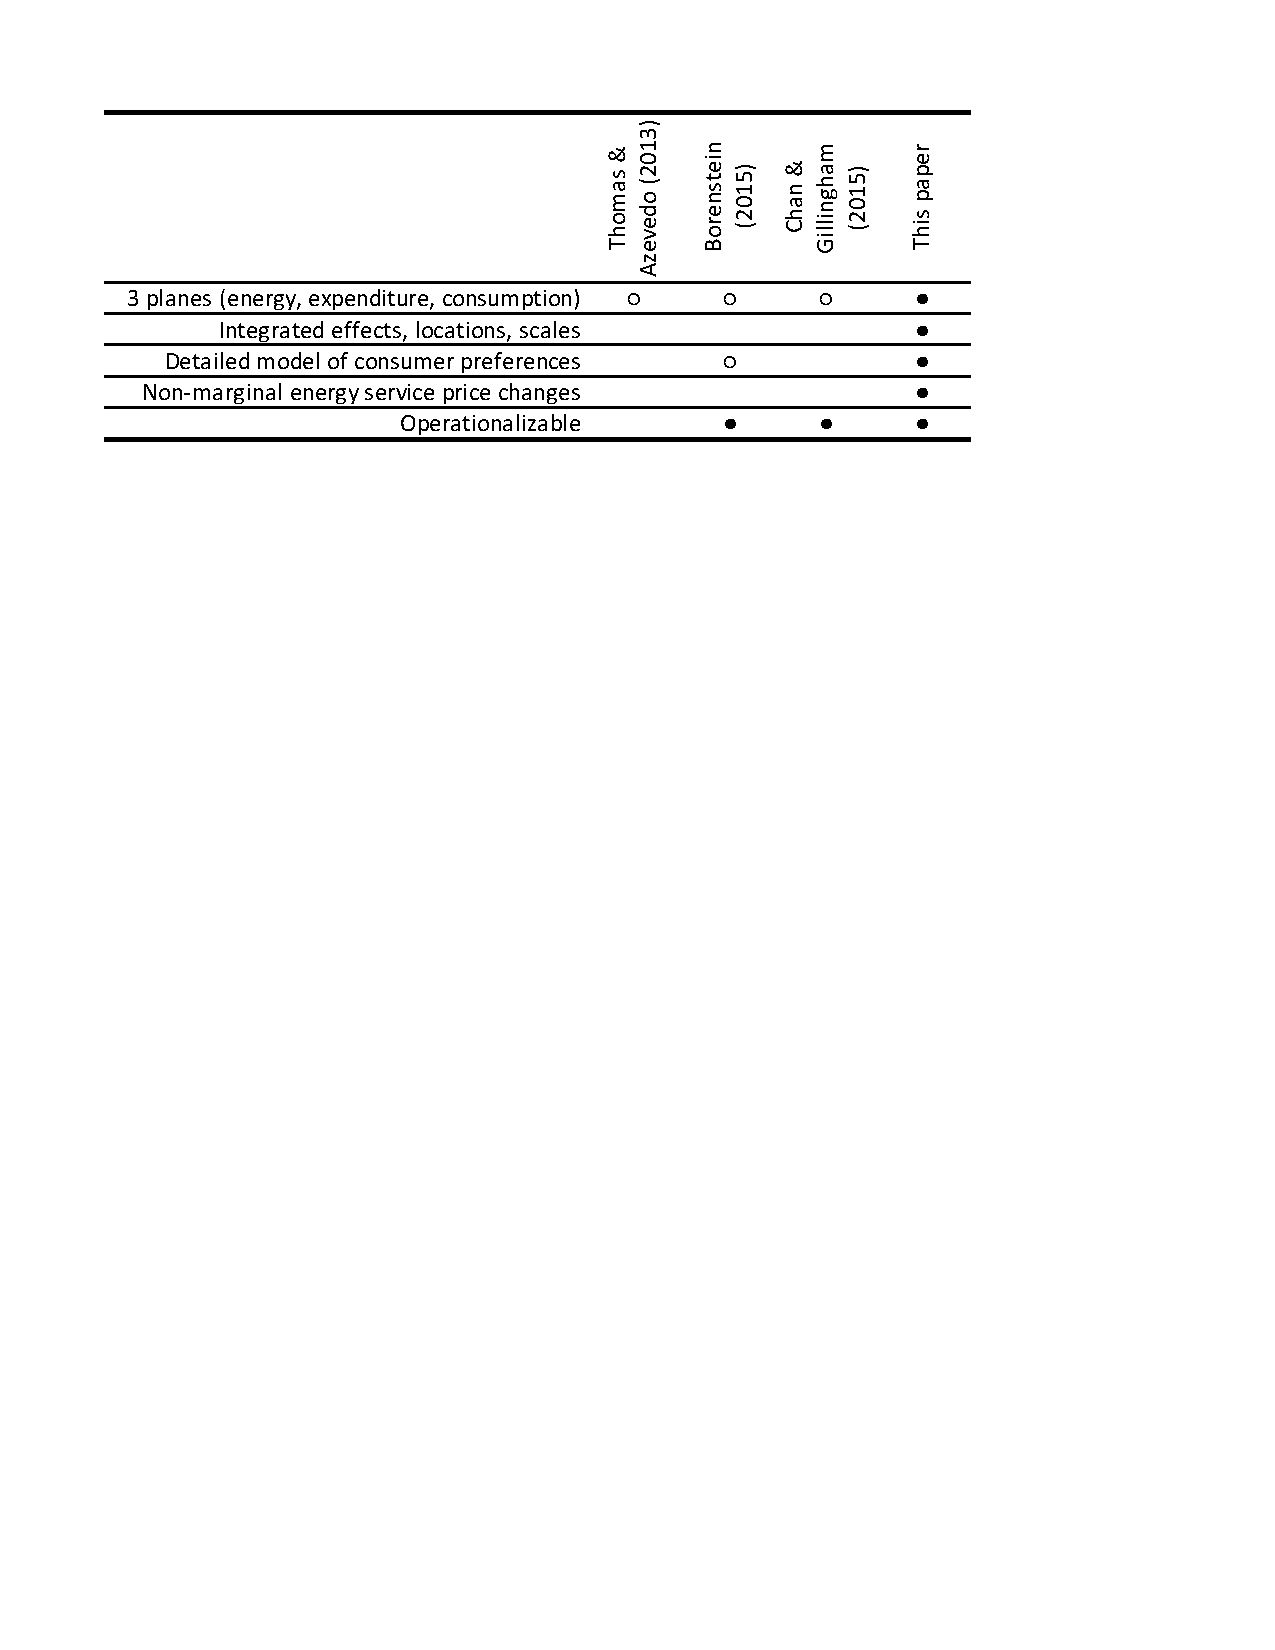
\includegraphics[width=1\linewidth]{figure_other/PreviousFrameworksTable.pdf}
%   \label{tab:previous_frameworks}
% \end{table}

